%!TEX root = /Users/markelikalderon/Documents/Git/formwithoutmatter/aristotle.tex
\chapter{Color} % (fold)
\label{cha:color}

\section{Aristotle's Explanatory Strategy} % (fold)
\label{sec:aristotle_s_explanatory_strategy}

At the opening of \emph{De Anima} \textsc{ii} 4\index{De Anima@\emph{De Anima}}, Aristotle describes an explanatory strategy\index{explanatory strategy} to be pursued in his subsequent discussion of the special senses\index{special senses} including color vision:
\begin{quote}
	It is necessary for the student of these forms of soul first to find a definition of each, expressive of what it is, and then to investigate its derivative properties, \&c. But if we are to express what each is, viz. what the thinking power is, or the perceptive, or the nutritive, we must go farther back and first give an account of thinking or perceiving; for activities and actions are prior in definition to potentialities. If so, and if, still prior to them, we should have reflected on their correlative objects, then for the same reason we must first determine about them, i.e. about food and the objects of perception and thought. (Aristotle, \emph{De Anima} \textsc{ii} 4 415\( ^{a} \)14--22\index{De Anima@\emph{De Anima}}; Smith in \citealt[26]{Barnes:1984uq})
\end{quote}
Perceptual capacities\index{capacity} are to be understood in terms of perceptual activities that are their exercise and what they are the potential for\index{capacity!explained in terms of exercise}. Thus sight\index{sight} is the perceiver's potential for seeing\index{seeing}. In seeing the perceiver exercises their capacity for sight. Moreover, seeing is what sight is the potential for. Sight is for the sake of seeing.\index{sight!for the sake of seeing} Aristotle's thought here is that potentialities\index{potential} are individuated by what they are the potential for, that for the sake of which the perceiver has the relevant capacity. Just as perceptual capacities are understood in terms of perceptual activities, perceptual activities are themselves to be understood in terms of their object. More specifically, perceptual activities are to be understood in terms of their primary object. The primary object\index{perception!object of!primary} of a given sensory modality must be perceptible to that sense alone and about which no error is possible, at least about its presence. The presentation\index{presentation} of the primary object in sense perception is what a sensory capacity is the potential for. Sight is, by its very nature, the potential to bring the colors of remote external particulars into view when it is light and to bring ``fiery or shining''\index{fiery or shining|seealso{the luminous}} (\emph{De Anima} \textsc{ii} 7 419\( ^{a} \)1--2)\index{De Anima@\emph{De Anima}} things into view when it is dark\index{dark}. Not every object of perception is a primary object\index{perception!object of!primary}. We can see motion\index{motion} and feel motion. But Aristotle maintains that we see motion only incidentally. By this he does not mean deny that motion is perceptible in itself---that would make motion an incidental and not a common sensible. His thought, rather, seems to be that sight is the potential for seeing colors in light and the fiery or shining in dark. This capacity enables us to see a variety of other objects as well. But sight is not for the sake of seeing motion\index{motion} or magnitude\index{magnitude}. Sight is for the sake of seeing color\index{color} in light\index{light} and the fiery or shining\index{the luminous} in dark\index{dark}. The non-primary objects of sight are incidental in the sense of being incidental to the nature of sight. The nature of sight as a potentiality is wholly determined by what it is a potential for, to present in visual consciousness colors in light and the fiery or shining in dark.

% section aristotle_s_explanatory_strategy (end)

\section{The Objects of Perception} % (fold)
\label{sec:the_objects_of_perception}

Among the objects of perception, Aristotle distinguishes three kinds (\emph{De Anima} \textsc{ii} 6):
\begin{enumerate}[(1)]
	\item primary sensibles,\index{perception!object of!primary}
	\item common sensibles, and\index{perception!object of!common}
	\item incidental sensibles.\index{perception!object of!incidental}
\end{enumerate}
Not only is color an object of sight but it is a primary object of sight as well.\index{color!primary object of sight} According to Aristotle's avowed explanatory strategy\index{explanatory strategy}, the primary objects of perception enjoy a certain explanatory priority\index{perception!object of!primary}. Once we better understand the sense in which color is a primary object of perception, we will better understand color's explanatory role---an explanatory role that, as we shall see, places a substantive constraint on a coherent interpretation of Aristotle's definition of color\index{color!definition}.

Aristotle's threefold distinction is presented as if it were a partition on the objects of perception. However, according to Aristotle, we perceive more than the primary\index{perception!object of!primary}, common\index{perception!object of!common}, and incidental\index{perception!object of!incidental} sensibles. For example, we perceive the difference in kind between primary objects---we perceive the difference between color\index{color} and sound\index{sound}, say. While we perceive such differences, Aristotle never describes these as a further kind of sensible. This raises an apparent puzzle. Aristotle explains the object of perception as what is perceived. Sensibles, being objects of perception, would just be whatever is perceived. But among what is perceived is a difference in kind between primary objects that is not itself a sensible. How are we to understand this? 

Here, I think it is useful to recognize a certain complexity in the structure of our perceptual capacity as Aristotle conceives of it. The human perceptual capacity at least comprises the five special senses\index{special senses}. The threefold distinction between primary\index{perception!object of!primary}, common\index{perception!object of!common}, and incidental\index{perception!object of!incidental} sensibles holds among the objects of the special senses. But the perception of difference between the primary objects of distinct senses could not be explained by the capacities involved in the special senses alone. Rather, the perception of difference involves a further perceptual capacity. So the human perceptual capacity, as understood by Aristotle, comprises not just the capacities involved in the five special senses, but comprises other perceptual capacities as well. The puzzle is resolved once we recognize that the threefold distinction constitutes a partition of the objects of the special senses. But as perception involves further perceptual capacities, what is perceived is not itself confined to the objects of the special senses\index{special senses}. What is perceived but not by the special senses is explained by the operation of a further perceptual capacity \citep[see][33--34]{Gregoric:2007yq}\index{Gregoric, Pavel}.

Aristotle's threefold distinction of the objects of the special senses is the result of two more fundamental distinctions and their interrelationship. Thus Aristotle distinguishes between:
\begin{enumerate}[(i)]
	\item objects that are perceptible in themselves\index{perceptible!in themselves}, and
	\item objects that are not perceptible in themselves but only incidentally perceptible.\index{perceptible!incidentally}
\end{enumerate}

Objects that are perceptible in themselves\index{perceptible!in themselves} are causes of perception in virtue of what they are. They contain within themselves the power of their own perceptibility. For example, color\index{color}, being what it is, is of such a nature that, in certain conditions, it can mediately act upon the organ of sight\index{sight} in such a way that the animal perceives that color. Objects that are not perceptible in themselves but only incidentally perceptible\index{perceptible!incidentally} are not causes of perception in virtue of what they are. Rather, they are perceived not in virtue of what they are but in virtue of their incidental relation to things that are perceived in themselves. Thus one can see the son of Diares\index{son of Diares} by seeing a white\index{white} object.

Some commentators have suggested that the paleness of the son of Diares\index{son of Diares} is a class signifier, a stereotypical observable feature of philosophy students who do not labor under the sun\index{sun}. While this would link Aristotle's example to certain aspects of classical literature, nevertheless I believe that Aristotle is inviting us to visually imagine the son of Diares seen from a great distance. Should he be wearing a white chiton, say, from a great distance, the son of Diares would appear as a white speck. 

The son of Diares\index{son of Diares} is an incidental sensible\index{perception!object of!incidental}. The son of Diares is a substance\index{substance}. Are ordinary material substances, such as a tomato\index{tomato} one might see at a supermarket, incidental sensibles\index{perception!object of!incidental}? One cause for caution is the indirect description of the unnamed man. Even if one were in a position to see that man, one may nevertheless remain in the dark that the man that one was seeing was in fact the son of Diares\index{son of Diares}. If in this way the son of Diares is a distant ancestor of Ortcutt\index{Ortcutt}, then Aristotle's example of an incidental sensible is not a substance, the individual man whose father was Diares, but an instance of the relational property, being the son of Diares. So understood, being the son of Diares is not sensible in these circumstances the way that his whiteness\index{white} is. Nevertheless the son of Diares\index{son of Diares} is perceptible by being incidentally related to what is perceptible in itself, the presented whiteness. The relation to his color is incidental since he might have presented some other color consistent with being the son of Diares. He might have worn a chiton of a different color.

It is difficult to determine Aristotle's precise understanding of incidental sensibles\index{perception!object of!incidental}. While he gives us an abstract characterization of incidental sensibles as perceptible not in themselves but by being incidentally related to things that are perceptible in themselves, he does not list or otherwise elaborate what incidental sensibles are. This masks potential difficulties. For example, perhaps it is plausible that some things are perceptible but not in themselves, but by being incidentally related to things that are perceptible in themselves. But it does not follow that all things incidentally related to things perceptible in themselves are perceptible. Seventeen is incidentally related to Benacerraf\index{Benacerraf, Paul} as his favorite number. Benacerraf is perceptible. Does it follow that seventeen is incidentally perceptible? If not, we are owed an explanation of how the line is drawn.

One final remark about the perception of ordinary material substances\index{substance}, or object perception\index{object perception} in modern parlance. Suppose that ordinary material substances are neither primary\index{perception!object of!primary}, nor common\index{perception!object of!common}, nor incidental\index{perception!object of!incidental} sensibles. Given that Aristotle's threefold distinction holds, not of the objects of perception, but of the objects of the special senses, it would not follow that we do not perceive ordinary material substances. The difference between the primary objects of the special senses\index{special senses} is perceptible but is not itself the object of any of the special senses. I suspect that a failure to appreciate this point in the postwar Anglophone commentary is due to the influence of a then dominant philosophy of perception, the sense-datum theory\index{sense-datum theory}. The Aristotelian primary objects more or less become, in the seventeenth century, secondary qualities\index{secondary qualities} (more or less since, for example, the ``fiery or shining''\index{the luminous} drops out of view). And in the early twentieth century, these become sense data. Approaching Aristotle's text with the sense-datum theory as a background, it would be very tempting to think that we are presented with colors\index{color}, sounds\index{sound}, and tastes\index{taste}---sense data---and that we are not presented with ordinary material objects, at least not directly, in perceptual experience. However, such a reading is anachronistic and is not born out by the text.

Among objects that are perceptible in themselves, Aristotle distinguishes between:
\begin{enumerate}[(a)]
	\item objects that are perceptible to one sense alone, and\index{perceptible!to one sense alone}
	\item objects that are perceptible to more than one sense.\index{perceptible!to more than one sense}
\end{enumerate}
Thus we can see colors\index{color}, hear sounds\index{sound}, and taste\index{taste} flavors\index{flavor}, but these sensory objects are available to no other sensory modalities. These are the primary sensibles\index{perception!object of!primary}. In contrast, we can see the motion\index{motion} and magnitude\index{magnitude} of a sensible particular and feel that motion and magnitude. These are common sensibles\index{perception!object of!common}. Common sensibles are common precisely in being perceptible to more than one sense. So understood, the common sensibles are perceptible in themselves, they are causes of perception in virtue of what they are. It is just that common sensibles, being what they are, can cause perception via distinct sensory modalities.

We are now in a position to understand how these pair of distinctions and their interrelationship results in Aristotle's threefold distinction. Objects of the individual senses are either perceptible in themselves (i) or only incidentally perceptible (ii). This latter category consists of the incidental sensibles (3). Among the objects of perception that are perceptible in themselves (i) some are perceptible to one sense alone (a). These are the primary objects of sense (1). Objects that are perceptible in themselves (i) but to more than one sense (b) are the common sensibles (2). See Figure~\ref{fig:special}.

\begin{figure}[ht]
    \begin{center}
		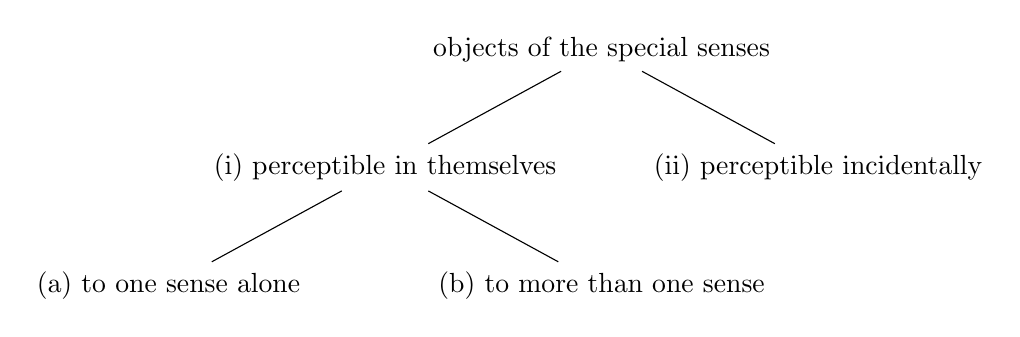
\begin{tikzpicture}
			\tikzstyle{level 1}=[sibling distance=5.5cm]
			\tikzstyle{level 2}=[sibling distance=5.5cm]
    		\node{objects of the special senses}
					child { node {(i) perceptible in themselves}
						child { node {(a) to one sense alone} }
						child { node {(b) to more than one sense} } }
					child { node {(ii) perceptible incidentally} }
			;
		\end{tikzpicture}
    \end{center}
	\caption{Objects of the special senses}
    \label{fig:special}
\end{figure}

However, when Aristotle defines primary objects of perception (\emph{De Anima} \textsc{ii} 6 418\( ^{a} \)11--12)\index{De Anima@\emph{De Anima}}, he does not restrict himself to the condition that they are perceptible in themselves to one sense alone. The primary objects\index{perception!object of!primary} of sense must meet a further condition: 
\begin{enumerate}[(1)]
	\item primary objects of a sense must be perceptible in themselves to that sense alone;
	\item no error is possible about the presence of the primary objects.
\end{enumerate}
Both conditions, but especially the second, require elaboration. 

However, the mere presence of the second condition itself raises a puzzle, whatever its content, given that the first condition suffices, by itself, to pick out the class of primary sensibles\index{perception!object of!primary}. The threefold distinction on the objects of the special senses is, as we have seen, the result of Aristotle's distinctions between what are perceptible in themselves\index{perceptible!in themselves} and what are incidentally perceptible\index{perceptible!incidentally}, and among what are perceptible in themselves, what are perceptible to one sense alone and what is perceptible to more than one sense. The taxonomy provided by Aristotle's two distinctions and their interrelationship would appear to be complete. But the first condition in his definition of primary objects just is their characterization in that taxonomy, thus rendering any second condition superfluous. To be sure, any second condition on the primary object of sense would be superfluous from the perspective of extensional adequacy. All and only primary objects of sense satisfy the first condition. But it would only follow that the second condition is superfluous if definition were solely concerned with extensional adequacy, but this is hardly the case for Aristotle. The second condition may not be needed to pick out the class of primary sensibles, but, as we shall see, it nevertheless reveals something important about the nature of the perceiver's relation to the primary object of their perceptual experience.

Aristotle inherits the first condition on being a primary object\index{perception!object of!primary}---that it be perceptible to one sense alone---from Plato's\index{Plato} discussion of perception in the \emph{Theaetetus}:\index{Theaetetus@\emph{Theaetetus}}
\begin{quotation}
	\textsc{socrates}: And are you also willing to admit that what you perceive through one power, you can't perceive through another? For instance, what you perceive through hearing, you couldn't perceive through sight, and similarly what you perceive through sight you couldn't perceive through hearing?
	
	\textsc{theaetetus}: I could hardly refuse to grant that. (Plato, \emph{Theaetetus} 184\( ^{e} \)8--185\( ^{a} \)3; Levett and Burnyeat in \citealt[204]{Cooper:1997fk})
\end{quotation}
Notice that Plato\index{Plato} links objects being perceptible to one sense alone to a conception of the senses as powers or capacities. Two thoughts seem to be at work here: (1) that powers or capacities\index{capacity!individuated by their exercise} are individuated by their proper exercise, and (2) that the proper exercise of sensory capacities is the presentation of its primary object in sensory awareness (compare as well \emph{Republic} \textsc{v} 477--478). These two claims in conjunction with specific claims about the primary objects of vision and audition imply that sight just is the capacity to see color, and audition just is the capacity to hear sound. If that is right, then, at least in broad outline, the avowed explanatory strategy of \emph{De Anima}\index{De Anima@\emph{De Anima}} \textsc{ii} 4 has its roots in Aristotle's reading of the \emph{Theaetetus}\index{Theaetetus@\emph{Theaetetus}}. Of course, Aristotle departs from Plato in crucial ways. Plato\index{Plato} seems to limit sense perception to the presentation of the primary objects\index{perception!object of!primary} in sensory awareness. However, Aristotle allows the senses to present objects common to other sensory modalities, though this is incidental to their nature, a nature that wholly consists in their potential to present their proper objects. In allowing the senses to take as their object proper\index{perception!object of!primary} and common\index{perception!object of!common} sensibles, Aristotle is conceiving of the senses as powers or capacities that can have different exercises---seeing motion is the exercise of the perceiver's capacity for sight\index{sight} just as seeing color\index{color} is (see \citealt{Freeland:1986fp}\index{Freeland, Cynthia}). Their being as potentialities, however, depend solely on their proper exercise, the sensory presentation of their proper object. Plato\index{Plato}, in contrast, maintains that perceptual capacities have as their exercise only the presentation of their proper objects maintaining that what is ``common'' to the objects of the senses---that they are each the same and different from the others---is determined by cognitive, not perceptual, capacities (\emph{Theaetetus} 184)\index{Theaetetus@\emph{Theaetetus}}. This is the basis for a further difference. Aristotle maintains that we can discriminate among the presented objects of sense and that this is the exercise of perceptual, not cognitive, capacities (\emph{De Anima} \textsc{iii} 2 426\( ^{b} \)9--16)\index{De Anima@\emph{De Anima}}. For discussion of just how far Aristotle extends the perceptual domain as Plato conceives of it see \citealt{Sorabji:2003fk} as well as his earlier discussion \citealt{Sorabji:1971fr}.\index{Sorabji, Richard}

Common sensibles\index{perception!object of!common}, like primary objects\index{perception!object of!primary}, are perceptible in themselves\index{perceptible!in themselves}, they are causes of perception in virtue of what they are. It is just that common sensibles, being what they are, can cause perception via distinct sensory modalities. That the primary objects are perceptible to one sense alone is the fundamental difference between primary objects and common sensibles. It is a fundamental difference in that it is a manifestation of the explanatory priority of the primary objects of perception. Perceptual capacities are individuated by their distinctive kinds of object. If the presentation of a common sensible were, \emph{per impossible}, the proper exercise of a perceptual capacity, then the different senses to which it is available would be identified. If the presentation\index{presentation} of a sensory object is to be definitive of the perceptual capacity whose exercise it is, that object must be presented to that sense alone. This is manifest in a further related difference between primary and common sensibles. Primary and common sensibles are perceptible in themselves. Each are the ultimate efficient cause of their perception. However only the primary object is a final cause. Not only are colors the ultimate efficient cause of color perception, but they are the final cause as well. Sight is for the sake of seeing color\index{color} in light\index{light} and the ``fiery or shining''\index{the luminous} in dark\index{dark}. The nature of an individual sensory capacity wholly consists in their potential to present their primary objects. Sight\index{sight} is not for the sake of seeing motion\index{motion}, though motion may be presented in sight. Thus common sensibles while ultimate efficient causes are not themselves final causes.

That the primary objects\index{perception!object of!primary} are perceptible to one sense alone is the fundamental difference between primary objects and common\index{perception!object of!common} sensibles. It is the fundamental difference, but not, as we have seen, the sole difference. There is a further important difference. Whereas as error is possible about the common sensibles, no error is possible about the primary objects, at least about their presence. Not only must proper objects be perceptible in themselves and perceptible to one sense alone, but about their presence no error is possible. No error may be involved in a color being present in sight, though one may be mistaken about the location of the presented color. Indeed, Aristotle goes so far as to define primary objects not only in terms of being perceptible in themselves to one sense alone, but also in terms of the condition that about their presence no error is possible.

One striking thing about this condition is its negative characterization. This is potentially philosophically significant since there are two ways to understand this denial\index{error!two senses distinguished}. No error may be possible either in the sense that:
\begin{enumerate}[(1)]
	\item perceptions of primary objects are always true or correct; or
	\item perceptions of primary objects are not the kind of thing that can be true or false, correct or incorrect.
\end{enumerate}
If the perception of primary\index{perception!object of!primary} objects were always true or correct, then no error would be possible, at least about their presence. If, however, the perception of primary objects were not the kind of thing that so much as could be true or false, correct or incorrect, no error would be possible, but in a difference sense. The sensing of primary objects would be impervious to error not because of some guarantee that the primary objects of a sense falls within its ken but because the sensing of a primary object fails to be evaluable as correct or incorrect. This latter thesis is put forward by Kant\index{Kant, Immanuel}:
\begin{quote}
	Truth or illusion is not in the object, in so far as it is intuited, but in the judgment about it, in so far as it is thought. It is therefore correct to say that the senses do not err---not because they always judge rightly but because they do not judge at all. \emph{Kritik der reinen Vernunft}\index{Kritik der reinen Vernunft@\emph{Kritik der reinen Vernunft}} \textsc{a}294/\textsc{b}350
\end{quote}

While Aristotle's usual formulation in Book \textsc{ii} of \emph{De Anima}\index{De Anima@\emph{De Anima}} is that no error is possible about the presence of primary objects\index{perception!object of!primary}, he does sometimes say, especially in Book \textsc{iii} that the perception of primary objects is always true. This provides \emph{prima facie} support for the first interpretation. On this interpretation, sense perception has something like an intentional or representational content. It is at least evaluable as true or false, correct or incorrect. Against this suggestion, an advocate of the second interpretation might claim that, by itself, this leaves unexplained what needs explaining---\-Aristotle's apparent preference for the negative characterization in Book \textsc{ii}. Aristotle's preference for the negative characterization is well explained by the second interpretation. On that interpretation, the denial of the possibility of error is not consistent with perceptions being always true, and so the condition could only be expressed by the negative characterization. The problem for the second interpretation is the potential embarrassment of explaining away the claim that the perception of primary objects is always true as merely loose talk if not indeed a slip on Aristotle's part.

We can decide between these rival interpretations by considering Aristotle's account of error (\emph{De Anima} \textsc{iii} 3 428\( ^{b} \)17-26, 430\( ^{a} \)27--430\( ^{b} \)5)\index{perception!object of!primary}. According to Aristotle, error\index{error} requires a certain kind of complexity, a complexity that the sensory presentation of the primary\index{perception!object of!primary} objects lacks. Specifically, only with combination\index{combination} is error\index{error!account of} possible:
\begin{quote}
	\ldots\ where the alternative of true or false applies, there we always find a sort of combining of objects of thought in a quasi-unity. As Empedocles said that ``where heads of many a creature sprouted without necks'' they afterwards by Love’s power were combined, so here too objects of thought which were separate are combined \ldots\ (Aristotle, \emph{De Anima} \textsc{iii} 6 430\( ^{a} \)27--32\index{De Anima@\emph{De Anima}}; Smith in \citealt[54]{Barnes:1984uq})
	
	For falsehood always involves a combining; for even if you assert that what is white is not white you have combined not-white. (Aristotle, \emph{De Anima} \textsc{iii} 6 430\( ^{b} \)1--3; Smith in \citealt[54]{Barnes:1984uq})
\end{quote}
(See also \emph{Categoriae} \textsc{ii} 1\( ^{a} \)16\index{Categoriae@\emph{Categoriae}}, \emph{De Interpretatione} \textsc{i} 16\( ^{a} \)9--18, \textsc{v} 17\( ^{a} \)17--20)\index{De Interpretatione@\emph{De Interpretatione}}, and the \emph{Sophist} 262\index{Sophist@\emph{Sophist}}.) The simple presentation of the white\index{white} of the sun\index{sun}, when not combined with other sensible elements of the scene, is not in error. But not because of any guarantee that color perception is always true. Rather, it is only when sensible objects are combined that the senses may mislead. We cannot be mistaken about the presence of the sun's\index{sun} whiteness\index{white} upon seeing it, but we can be mistaken about the location of the whiteness, when we combine whiteness, a primary object\index{perception!object of!primary}, with other sensibles, such as location\index{location}, in this case, a common sensible\index{perception!object of!common}. Since the sensory presentation\index{presentation} of primary objects does not involve combination\index{combination}, and combination is necessary for error, then no error is possible about the presence of these sensory objects in the strong sense that their perception is not the kind of thing that so much as could be evaluable as true or false, correct or incorrect.\index{perception!object of!primary!no error is possible} In sensory consciousness we simply confront the primary object of the given modality. We cannot be confronted truly or falsely, correctly or incorrectly. We simply confront what is presented to us in sensory consciousness. 

This is the basis for the second contrast that Aristotle draws between perception\index{perception!contrasted with understanding} and understanding in the following passage from Book \textsc{iii} of \emph{De Anima}:
\begin{quote}
	That perceiving and understanding are not identical is therefore obvious; for the former is universal in the animal world, the latter is found in only a small division of it. Further, thinking is also distinct from perceiving---I mean that in which we find rightness and wrongness---right\-ness in understanding, knowledge, true opinion, wrongness in their opposites; for perception of the special objects of sense is always free from error, and is found in all animals, while it is possible to think falsely as well as truly, and thought is found only where there is discourse of reason. (Aristotle, \emph{De Anima} \textsc{iii} 3 427\( ^{b} \)7--15\index{De Anima@\emph{De Anima}}; Smith in \citealt[49]{Barnes:1984uq})
\end{quote}
All animals\index{animal} perceive\index{perception}, but not all animals are rational\index{animal!rational}. Rational activity, such as thinking\index{thinking}, is evaluable as correct or incorrect. But perceptions of primary objects\index{perception!object of!primary}, being simple presentations\index{presentation} of these sensory objects, are insusceptible to error in this way\index{error}. The line of reasoning behind this way of contrasting perception and understanding can be found in the \emph{Theaetetus}\index{Theaetetus@\emph{Theaetetus}}, on at least some interpretations (see \citealt{Cooper:1970kx}\index{Cooper, John} and \citealt{Burnyeat:1990dp}\index{Burnyeat, M.F.}). So it is possible that the second condition on being a primary object itself derives from Aristotle's reading of the \emph{Theaetetus} as well.

% \citet{Caston:1998nx}\index{Caston, Victor}, while conceding that error\index{error} in judgment requires combination\index{combination}, maintains that Aristotle offers a different account of perceptual error. He does so on the basis of the following passage from \emph{De Insomniis}\index{De Insomniis@\emph{De Insomniis}}:
% \begin{quote}
% 	The ground of such false judgments is that any appearances whatever present themselves, not only when its object moves a sense, but also when the sense by itself alone is moved, provided only it be moved in the same manner as it is by the object. (\emph{De Insomniis} \textsc{ii} 460\( ^{b} \)23--25; Beare in \citealt[6]{Barnes:1984uq})
% \end{quote}
% If combination is only necessary for error in judgment, then it does not follow that the presentation of a primary object in sensory experience, being simple and hence no combination, is not in error in the sense of being not the kind of thing that can be assessed as correct or incorrect. However, no genuine alternative is offered here, that is, an account of error applicable specifically to sense experience and not involving combination the way that error in judgment does. To see this, it suffices to attend to the larger context from which the passage cited by Caston is drawn. The cited passage comes towards the end of an extended discussion that Aristotle inaugurates

The primary\index{perception!object of!primary} object of sight\index{sight} is the visible\index{the visible}. What is visible is either color\index{color} or ``a certain kind of object which can be described in words but which has no single name'' (\emph{De Anima} \textsc{ii} 7 418\( ^{a} \)26)\index{the luminous}. So color is a primary object of sight not the primary object of sight (though see \citealt[252]{Polansky:2007ly}\index{Polansky, Ronald} for a denial of the claim that that which has no name is a primary object of sight). That a sense can have a plurality of primary objects is consistent with Aristotle's two defining conditions on being a primary object---that it be perceptible in itself to one sense alone and about whose presence no error is possible. Distinct kinds of objects can each satisfy these conditions. So it does not follow from Aristotle's definition of primary objects that for each sense there is exactly one primary object. If there is a problem, especially if, as in the case of touch, there are too many primary objects, this must be due not solely to the definition of primary object but must involve as well further explanatory assumptions. As we shall see, any difficulty posed by a plurality of primary objects is due less to the definition of primary object than to the explanatory role they play in Aristotle's avowed strategy of explaining perceptual capacities in terms of perceptual activities and explaining perceptual activities in terms of their primary objects.

Colors\index{color} depend upon light\index{light} for their visibility. But not everything depends upon light for their visibility. That which has no name does not so depend\index{the luminous}:
\begin{quote}
	Some objects of sight which in light are invisible, in darkness stimulate the sense; that is, things that appear fiery or shining. This class of objects has no simple common name, but instances of it are fungi, horns, heads, scales, and eyes of fish. In none of these is what is seen their own proper colour. Why we see these at all is another question. (Aristotle, \emph{De Anima} \textsc{ii} 7 419\( ^{a} \)2--7\index{De Anima@\emph{De Anima}}; Smith in \citealt[33]{Barnes:1984uq})
\end{quote}
Philoponus\index{Philoponus, John}, in his commentary on \emph{De Anima}, reports a slightly different list of examples:
\begin{quote}
	\ldots\ glow worms, heads of fish, fish scales, eyes of hedgehogs, shells of sea-creatures, which things are seen not in light but in dark. (Philoponus, \emph{On \emph{De Anima}} 319 25--27\index{On De Anima@\emph{On \emph{De Anima}}}; \citealt[3]{Charlton:2005fk})
\end{quote}
That which has no name possess qualities visible in the dark and not the light and differ from the proper colors of these same things which are visible in the light and not the dark. This is most likely the source of Austin's\index{Austin, J.L.} example from \emph{Sense and Sensibilia}\index{Sense and Sensibilia@\emph{Sense and Sensibilia}} (an appropriately Aristotelian title, at least in the present context):
\begin{quote}
	Suppose \ldots\ that there is a species of fish which looks vividly multi-coloured, slightly glowing perhaps, at a depth of a thousand feet. I ask you what its real colour is. So you catch a specimen and lay it out on deck, making sure the condition of the light is just about normal, and you find that it looks a muddy sort of greyish white. Well, is \emph{that} its real colour? \citep[lecture \textsc{vii}, 65--66]{Austin:1962lr}
\end{quote}
In the darkness\index{dark}, at the depth of a thousand feet, the fish\index{fish} may look vividly multi-colored and slightly glowing\index{bioluminescence}, but on the sun drenched deck they look a muddy sort of grayish\index{gray} white\index{white}. Aristotle would contend that only the latter is the creature's proper color, the former being an instance of that which has no name. Austin\index{Austin, J.L.} is, of course, making a different point with the Aristotelian example, that the ``real'' color of a thing may depend on the practical point of attributing color to it in the circumstances of saying.

There is a question about how broadly the domain of that which has no name extends\index{the luminous}. Some commentators have suggested that shining be interpreted as reflective\index{reflection} highlights. So fish scales\index{fish scales}, having a highly reflective surface, can produce highlights discernible even in conditions of very low illumination resulting in a shimmering effect set amidst the surrounding darkness. This interpretation is suggested by Aristotle's remarks in \emph{De Sensu}: 
\begin{quote}
	Things which are smooth have the natural property of shining in darkness, without, however, producing light. \ldots\ For it is in the dark that that which is smooth, e.g. the heads of certain fishes, and the sepia of the cuttle-fish, naturally shines \ldots\ (Aristotle, \emph{De Sensu} \textsc{ii} 437\( ^{a} \)31--437\( ^{b} \)5\index{De Sensu@\emph{De Sensu}}; Beare in \citealt[4]{Barnes:1984uq})
\end{quote}
The trouble with this interpretation is that it does not fit all of Aristotle's examples---fungi\index{fungi} lack smooth, reflective\index{reflection} surfaces and so give rise to no reflective highlights. One plausible thought, supported by Philoponus'\index{Philoponus, John} additional example of glow worms\index{glow worm}, and exploited by Austin\index{Austin, J.L.} in his appropriation, is that these are examples of bioluminescence\index{bioluminescence}. One minor problem with this interpretation is that the eyes of hedgehogs\index{hedgehog} glowing in a dark\index{dark} field---assuming, for the moment, that Philoponus'\index{Philoponus, John} example is of genuine Aristotelian provenance---are not radiant light\index{light} sources the way that they appear to be and the way that cases of  bioluminescence\index{bioluminescence} genuinely are. Rather, they are reflecting ambient light in circumstances of low illumination, say, from a lantern\index{lantern} of shaved horn held by an ancient spectator traversing the field at night. All of Aristotle's examples are biological, but the claim that that which has no name is visible in the absence of light suggests a generalization. After all, there are mineral deposits, of phosphorus\index{phosphorus}, say, whose glow can only be seen in the absence\index{absence} of competing illumination. So perhaps that which has no name includes not only the bioluminescent\index{bioluminescence}, but the luminous\index{the luminous} more generally. Philoponus\index{Philoponus, John} suggests this broader interpretation and provides the nice example of starlight\index{starlight}, visible only in the absence of the sun's\index{sun} light (\emph{On \emph{De Anima}} 347 11). 

It may be tempting to think that the difference between color\index{color} and the luminous\index{the luminous} as Aristotle conceives of it is the difference between, as we might put it, surface color and the color of radiant light sources. But this would be a mistake. Among the examples that Aristotle gives of colored particulars are radiant light sources, prominently, the sun\index{sun}. Moreover, if the defining feature of the luminous is its visibility in darkness, then, as our discussion has made clear, the luminous should include not only radiant light sources but reflections as well. The contrast between color and the luminous is not the contrast between surface color\index{color!surface} and radiant color\index{color!radiant}, but the contrast between light\index{light} and dark\index{dark} as conditions on the visibility of distinct kinds of objects.

Suppose then, that the two species of the visible\index{the visible} are to be understood in this way. Whereas color\index{color} is visible in the light\index{light}, the luminous\index{the luminous} is visible in the dark\index{dark}. One problem with Aristotle's view, so interpreted, is that the contrast does not constitute a partition and so could not demarcate two exclusive species\index{species} of visibilia\index{the visible}. Some things are visible in the light and the dark, as Philoponus\index{Philoponus, John} observes:
\begin{quote}
	For some of them are super-shining, some are dimly shining, and some middling. Those that are dimly shining are seen only at night, such as glow-worms\index{glow worm} and fish scales\index{fish scales} and the like; for their shining does not appear by day, being overcome by a greater. And also a majority of stars\index{stars}. Those that are middling are seen both at night and by day, such as the moon\index{moon} and some of the stars, for instance the Morning Star\index{Morning Star} when the sun is near the horizon and the Morning Star itself is near its perigee. Fire\index{fire} also. For this perfects air\index{air} so as to show also the colours that are in it, but in the rest it shows itself, indeed, but does not bring transparency to that part to actuality. Hence we see itself when we are a long way off in the dark, but none of the colours around us. By day, again, fire\index{fire} appears as something shining, but not as doing anything to the air because that is already affected by a greater shining, and then it appears in a way like the other colours, but more in the way of the shining of the moon\index{moon} also, because it is not too dim, appears by day; so also with the shining of fire, when it is shown not far away and it is light. But the super-shining are seen only by day, viz. the sun\index{sun}, since indeed it is the cause of day\index{day} and of light\index{light}. (Philoponus, \emph{On \emph{De Anima}} 347 7--24\index{On De Anima@\emph{On \emph{De Anima}}}; \citealt[32]{Charlton:2005fk})
\end{quote}

It is hard to know how Aristotle would address this difficulty since he gives no explanation for how the luminous\index{the luminous} may be visible in the dark\index{dark}. Recall, against Democritus\index{Democritus}, Aristotle argues, on general grounds (\emph{De Anima} \textsc{ii} 7 418\( ^{b} \)13--22)\index{De Anima@\emph{De Anima}}, that remote objects of perception require a medium\index{medium} if they are to act upon the perceiver's sense organ, which they must do since sensation is a mode of sensitivity, a reactive capacity. There is no action at a distance. Action, or at any rate immediate action, requires contact. But the remote objects, being remote, are not in contact with the perceiver's sense organ. But this is consistent with them acting upon the perceiver's sense organ mediately, by acting upon something else which is in contact, that is to say, by acting upon an intervening medium. The reasoning here is sufficiently general to hold true, as well, of seeing the luminous\index{the luminous} set amidst the surrounding darkness\index{dark}. Moreover, just as in the case of color vision, the medium\index{medium} is transparent\index{transparency}, the difference being that the medium, be it air\index{air} or water\index{water}, is potentially if not actually transparent. Exactly how, though, the luminous acts upon the potentially if not actually transparent, Aristotle declines to say, simply dropping the matter. Indeed, he proceeds to speak as if color were the sole primary object of sight. But exactly how the luminous acts upon the potentially if not actually transparent medium is an essential part of the explanation for how the luminous may be visible in the dark. In the absence of such an explanation, there is no saying what Aristotle might say about the formal difficulty raised by Philoponus'\index{Philoponus, John} observation. Aristotle must have been apprised of this difficulty since he makes the crucial observation himself:
\begin{quote}
	Fire on the other hand is seen both in darkness and in light; this double possibility follows necessarily from our theory, for it is just fire that makes what is potentially transparent actually transparent. (Aristotle, \emph{De Anima} \textsc{ii} 7 419\( ^{a} \)23--24\index{De Anima@\emph{De Anima}}; Smith in \citealt[34]{Barnes:1984uq})
\end{quote}
Though Aristotle makes the crucial observation upon which the apparent difficulty turns, he nonetheless expresses confidence that the difficulty is merely apparent. That fire\index{fire} is visible in the light\index{light} and dark\index{dark} is somehow meant to follow from the fact that it is fire that makes the potentially transparent actually transparent, though he never gives the relevant explanation.

Earlier I observed that a plurality of primary objects\index{perception!object of!primary!plurality} is consistent with Aristotle's two defining conditions on being a primary object of sense. If a difficulty is posed by a plurality of primary objects, this must be due to further explanatory assumptions, indeed assumptions linked to Aristotle's avowed explanatory strategy (\emph{De Anima} \textsc{ii} 4)\index{De Anima@\emph{De Anima}}. However, understood in this light, there is less a difficulty about the plurality of primary objects, nor even about their being large in number, than about their diversity. It is a lack of unity among a plurality of primary objects that is potentially puzzling in the context of Aristotle's explanatory strategy. 

This is what underlies Aristotle's contrasting attitudes towards vision\index{sight} and touch\index{touch}. The proper object of vision is the visible\index{the visible}, and there are two species\index{species} of visibilia. About this Aristotle is apparently sanguine, if not terribly forthcoming. But when it comes to the plurality of primary objects of touch\index{touch}, Aristotle remarks that this is a source of puzzlement (\emph{aporia})\index{aporia@\emph{aporia}}. The difference concerns the unity displayed by the visible and the diversity displayed by the tangible.\index{the visible!unity of}\index{the tangible!diversity of}

Color\index{color} is visible in the light\index{light} and the luminous\index{the luminous} is visible in the dark\index{dark}. Light is a fundamental condition for the visibility of color, just as dark is a fundamental condition for the visibility of the luminous. So understood light and dark are states of potentially transparent\index{transparency} media such as air\index{air} and water\index{water}, light being the state of the medium\index{medium} when it is actually transparent and dark being the state of the medium when it is not actually but only potentially transparent.\index{light!two senses distinguished} There is a related sense in which light\index{light} and dark\index{dark} are visible qualities of these states. Air\index{air} and water\index{water}, when actually transparent\index{transparency}, is light or bright, just as it is dark when it is not actually but only potentially transparent. Light or brightness is the color of the actually transparent (\emph{De Anima} \textsc{ii} 7 418\( ^{b} \)11-12; \emph{De Sensu} \textsc{iii} 439\( ^{b} \)1--2)\index{De Sensu@\emph{De Sensu}}; and so dark is the color of what is not actually transparent. Moreover, so understood, light and dark are themselves united as opposing contraries. Contrast sensible qualities from different opposing pairs of contraries, light and loud, say. Furthermore, the opposing pair of contraries, light and dark, have a common determinant, the presence or absence, respectively, of the fiery substance\index{fiery substance} in a potentially transparent medium. So conceived, the visible displays a kind of unity. Moreover, the ``kinship'' between color and the luminous is metaphysical and not, or not primarily, phenomenological, as \citet[63]{Sorabji:1971fr} suggests.\index{the visible!unity of}

The tangible\index{the tangible}, in contrast, is remarkable and potentially puzzling because of the diversity of its objects.\index{the tangible!diversity of} ``Touch, indeed discriminates more than one set of different qualities'' (\emph{De Anima} \textsc{ii} 6 418\( ^{a} \)14\index{De Anima@\emph{De Anima}}; Smith in \citealt[32]{Barnes:1984uq}). The tangible\index{the tangible} comprises a variety of opposing pairs of sensible qualities, including hot\index{hot} and cold\index{cold}, dry\index{dry} and wet\index{wet}, hard\index{hard} and soft\index{soft}, and so on. And it is the apparent lack of unity among these opposing pairs of contraries that is the source of puzzlement. Aristotle illustrates this apparent lack of unity by contrasting the tangible\index{the tangible} with the audible\index{the audible}. There are a plurality of opposing pairs of contraries\index{contraries} that qualify the audible---sharp\index{sharp} and flat\index{flat}, loud\index{loud} and soft\index{soft}, smooth\index{smooth} and rough\index{rough}, and so on---but these are all intelligibly qualities of a single substratum, sound\index{sound!as substratum of audible qualities}. ``Nevertheless we are unable clearly to detect in the case of touch what the single subject is which corresponds to sound in the case of hearing'' (\emph{De Anima} \textsc{ii} 11 422\( ^{b} \)31--32\index{De Anima@\emph{De Anima}}; Smith in \citealt[40]{Barnes:1984uq}). We need not suppose that the requisite unity necessarily takes the form it does in the case of audibilia\index{the audible}, that the plurality of opposing pairs of contraries are united by a common substratum. After all, the unity of the visible was not achieved in this way. All that is required is that the plurality of primary objects be united in a manner sufficient to discharge their explanatory role. So what is puzzling is not the plurality of primary objects of touch, nor their being large in number, but the apparent lack of unity displayed among the primary objects of touch.

The diversity of the tangible\index{the tangible!diversity of} is puzzling\index{aporia@\emph{aporia}} when set in the context of Aristotle's avowed explanatory strategy. Aristotle is seeking definitions of each of the soul's capacities, such as an animal's cognitive, perceptual, and nutritive capacities, that are ``expressive of what it is''. Capacities\index{capacity} are a species of potentiality.\index{potential} What a capacity is depends upon what it is a potential for. What makes sight sight\index{sight} is that it is a potential for seeing\index{seeing}. Given the special nature of perceptual and epistemic activities---they each take an object---a definition of perceptual activity expressive of what it is would make essential reference to its object. Seeing is sensory awareness of color\index{color} just as hearing\index{audition} is sensory awareness of sound\index{sound}. And it is their primary\index{perception!object of!primary} objects that distinguish these perceptual activities. If the primary objects of sense are to play this explanatory role, if perceptual activities are to be understood in terms of the presentation of these objects, and perceptual capacities are to be understood in terms of the perceptual activities that are their proper exercise, then primary objects of a given sense, if they constitute a plurality, must display sufficient unity to play this explanatory role.\index{explanatory strategy} Diversity among them would, within this framework, naturally lead one to wonder whether there really was one sensory modality at work here rather than many. Why should there be a single sense that affords awareness of hot and cold, wet and dry, hard and soft, rather than there being separate senses of temperature, moisture, and texture? This is precisely the puzzlement that inaugurates Aristotle's discussion of touch in \emph{De Anima} \textsc{ii} 11\index{De Anima@\emph{De Anima}}.

The unity of the visible\index{the visible!unity of} bears on the significance of Aristotle's declining to explain the visibility of the luminous\index{the luminous}. In a cynical mood, it is tempting to understand Aristotle's begging off as the expression of embarrassment at not having an adequate explanation. On this understanding, it is at least an open question whether there is an adequate explanation to be had. However, the unity of the visible makes it possible to understand Aristotle's declining to explain the visibility of the luminous in a different way. Rather than an expression of embarrassment, Aristotle's begging off is the expression of confidence that an explanation of the visibility of the luminous, consistent with the general principles at work in his explanation of the visibility of color\index{color}, is possible. And it is the unity of the visible, that which unites color with the luminous, being qualities whose visibility is determined by the presence or absence of the fiery substance\index{fiery substance} in potentially transparent\index{transparency} media\index{medium}, that is the grounds of such confidence. Aristotle's habit of speaking as if color is the sole primary object of sight\index{color!primary object of sight} can be understood as the expression of this confidence, grounded in the unity displayed by the plurality of the visible\index{the visible!unity of}. Without pausing to consider further whether this confidence is misplaced, we shall follow Aristotle in speaking as if color were the sole primary object of sight.

% section the_objects_of_perception (end)

\section{The Definition of Color} % (fold)
\label{sec:the_definition_of_color}

Aristotle's explanatory strategy\index{explanatory strategy} also importantly constrains the interpretation of his definition of color\index{color!definition}. Color is the primary object of sight\index{color!primary object of sight}. Given, Aristotle's avowed explanatory strategy, color, so understood, must be defined independently of color perception.

Before we consider Aristotle's definition, let us first briefly consider a small puzzle about the order of Aristotle's exposition of the special senses\index{special senses}. Aristotle's usual method of exposition would be to discuss the more fundamental of the special senses first. And touch\index{touch!fundamental} is fundamental in the sense that it is essential to all animals. Not all animals see, but all animals have the sensory capacity for touch. So on the usual method of exposition, one would expect Aristotle to begin his discussion of the special senses, not with sight\index{sight} and color\index{color} as he does, but with touch\index{touch} and the tangible\index{the tangible}. Why does Aristotle depart from the usual method of exposition? What is its significance? One idea is that Aristotle discusses the distal sense of sight first to motivate the need for an intervening medium\index{medium} before controversially arguing that a medium is in play in touch as well. That idea is plausible, so far as it goes, but it gains significance once we realize that Aristotle's order of exposition is dictated by his response to Empedoclean puzzlement. It is our perception of the colors inhering in remote external particulars that is the original source of such puzzlement. Color perception is meant to be problematic in the way that touch could not be. The departure from the usual method of exposition is the result of the consequent focus on color perception, and Aristotle will argue that touch, and not color perception, is the puzzling sensory modality (see chapter~\ref{sec:against_the_empedoclean_principle}).

Aristotle defines color\index{color!definition} as the power to move what is actually transparent (\emph{De Anima} \textsc{ii} 7 418\( ^{a} \)31--418\( ^{b} \)33; \textsc{ii} 7 419\( ^{a} \)10--12). Aristotle's definition, despite its brevity, has several distinguishable components. Specifically, in his definition, Aristotle distinguishes:\index{color!definition!components distinguished}
\begin{enumerate}[(1)]
	\item a power to effect change---color,\index{color!definition!power to effect change}
	\item a patient of change, that which color acts upon---transparent media,\index{color!definition!patient of change}
	\item a change that colors effect when acting upon transparent media---unspecified, and\index{color!definition!unspecified change}
	\item  a condition on the media being acted upon by color---that the media be actually transparent.\index{color!definition!condition on patient}
\end{enumerate}

Let me make some preliminary remarks about each of these components. Some of these are observations, while others have a more aporetic character, raising issues or difficulties, directly or indirectly related to color's explanatory role given Aristotle's avowed explanatory strategy, in \emph{De Anima}, of explaining perceptual capacities in terms of the perceptual activities that are their proper exercise, and explaining perceptual activities that are the proper exercise of our perceptual capacities in terms of the presentation of primary objects.
\begin{enumerate}[(1)]
	\item First, color is a power of external particulars, a power that is exercised in moving what is actually transparent.\index{color!definition!power to effect change} A particular may possess this power even when it is not exercised---when the medium\index{medium} is potentially but not actually transparent\index{transparency}, say, or when the particular is occluded\index{occlusion} from view by being an interior part of a body. It is thus a kind of potentiality, or at least the grounds for one. This is metaphysically significant since it implies that particulars retain their colors even when they are unseen, when in the dark\index{dark} or occluded\index{occlusion} from view, say. As I argued in chapter~\ref{cha:perception_at_a_distance}, Aristotle uses the actual/potential distinction to sustain a perceptual realism\index{realism}\index{color!realism}. Aristotle's definition would be the basis for distinguishing actual and potential color, potential color being the power to move what is actually transparent and actual color being that power's exercise, the moving of what is actually transparent. And indeed Aristotle is keen to distinguish actual and potential color. We have already seen an example of this in the \emph{De Sensu}\index{De Sensu@\emph{De Sensu}} discussion of opacity\index{opacity} (chapter~\ref{sec:transparency_in_de_sensu}). Moreover, towards the end of an important passage (\emph{De Anima} \textsc{iii} 2 426\( ^{a} \)2--26), Aristotle criticizes ``earlier students of nature''\index{earlier students of nature} for failing to distinguish actual and potential color. It is only in failing to distinguish actual and potential color that they maintain that without sight there is no color. Among the earlier students of nature, Aristotle thus undoubtedly has Protagoras\index{Protagoras} in mind. However, in Book \textsc{iii}, actual colors are the colors seen. The actual/potential contrast as drawn by Aristotle's Book \textsc{ii} definition is between the power to move what is transparent and its exercise. But color\index{color!definition!power to effect change} can move what is actually transparent and, in so moving, be visible in that medium and yet not be seen because there is no suitably placed, awake, and attentive perceiver. This need not be a problem. After all the actual and potential are said of in many ways. But it does raise a question about how Aristotle is understanding actual and potential color. Moreover, if, as the criticism of the earlier students of nature can seem to suggest, colors are most fully actual when perceived, it is at least not obvious that the colors are independent of perception in the way that is required by Aristotle's avowed explanatory strategy.
	\item Second, color is the power to move what is actually transparent. It is illuminated media that color acts upon.\index{color!definition!power to effect change} Color could not act upon the perceiver's organ of sight, at least not directly, since contact precludes sensation, to be palpable is to be imperceptible. Thus was the moral of Aristotle's criticism of the Empedoclean principle. While colors could not act upon the perceiver's sense organ, at least not immediately, they can nevertheless act upon the sense organ mediately, by acting upon an intervening medium. So this aspect of Aristotle's definition of color, that color acts upon an intervening medium as opposed to the organ of sight, is a direct consequence of his case against Empedocles. The contrast is usefully, if anachronistically, brought out as follows. Colors are powers. At least in this abstract regard, they are like Lockean\index{Locke, John} secondary qualities\index{secondary qualities}, on one philosophically influential interpretation. However, whereas Lockean secondary qualities are powers to elicit ideas in perceivers, colors, as conceived by Aristotle, are powers not to affect perceivers, but to affect something else, an illuminated medium, itself disposed to affect perceivers. So conceived, colors may be powers, but they are less like Lockean secondary qualities than they are like, in the traditional post-Lockean vocabulary, tertiary qualities\index{tertiary qualities}. Locke characterizes these qualities as follows: 
\begin{quote}
	The \emph{Power} that is in any Body, \emph{by} Reason of the particular Constitution of \emph{its primary Qualities}, to make such a \emph{change} in the \emph{Bulk, Figure, Texture and Motion of another Body}, as to make it operate on our Senses differently from what it did before. (Locke, \emph{An Essay Concerning Human Understanding} \textsc{ii} 8 23)
\end{quote}
Locke's (\emph{An Essay Concerning Human Understanding} \textsc{ii} 8 23) own examples of tertiary qualities are ``the Sun has a Power to make Wax white, and Fire to make Lead fluid''.\index{sun}\index{white}\index{wax} If colors were powers to affect illuminated media, then colors would be Lockean tertiary qualities\index{tertiary qualities}, at least on a reasonable generalization of that notion. Color, so conceived, would be the power of external particulars, by reason of their particular elemental composition\index{elements}, to make such a change to the illuminated medium\index{medium} so as to make it operate on our sense of sight differently from what it did before. (``Before'', here, should be understood as a temporal metaphor for a modal claim---the illuminated medium affected by the color of a particular operates on color vision differently from the way it would if it were not affected by that particular's color.) Colors, as conceived by Aristotle, are ways of affecting light.\index{color!definition!power to effect change}
\item Third, as \citet[367]{Hicks:1907uq}\index{Hicks, R.D.} observes, by motion\index{motion} Aristotle does not mean locomotion\index{locomotion} or change in position. Rather, in \emph{De Anima}\index{De Anima@\emph{De Anima}}, \emph{kin\={e}sis} is Aristotle's general term for change\index{change} of any kind. Thus motion in Aristotle's definition means productive of change rather than productive of spatial movement, more narrowly. Frustratingly, Aristotle does not directly specify the nature of the change color induces in the transparent medium it acts upon. Indeed, in \emph{De Anima} \textsc{ii} 7 the only effect of color discussed is the effect in terms of which the transparent is defined\index{transparency!definition}---the transparent is not visible in itself, but owing its visibility to the color of another thing. Is this change, the rendering visible of the transparent, sufficient to understand Aristotle's definition? If it were, this would explain Aristotle's apparent silence about the nature of the change induced in the transparent by color---he merely says nothing further, having already specified the nature of the change in his definition of the transparent. Is this credible? What are the alternatives?\index{color!definition!unspecified change}
\item Fourth, the medium\index{medium} must meet a certain condition\index{color!definition!condition on patient} for color to act upon it---it must be actually transparent\index{transparency}. A doubt may be registered about the occurrence of transparency in Aristotle's definition\index{transparency!definition} given his avowed explanatory strategy\index{explanatory strategy}. Color is a proper object of sight\index{color!primary object of sight}, and, as such, partly defines the nature of sight\index{sight}. It might reasonably be thought that color could only play a role in defining sight if it had a nature independent of sight. But defining color in terms of the power to move what is actually transparent potentially threatens this order of explanation given the definitional connection between transparency and visibility. It is on these grounds that \citet{Zabarella:1605kx}\index{Zabarella, Jacopo} rejects Aristotle's definition \citep[see][for discussion]{Broackes:1999uq}\index{Broackes, Justin}.
\end{enumerate}

Begin with the one known effect that color has on what is actually transparent,\index{transparency} the rendering visible of the transparent. What is actually transparent is illuminated by the presence and activity of the fiery substance. Aristotle's idea is that we see the illuminated media by seeing the colored particulars arrayed in it. In chapter~\ref{cha:transparency}, I motivated Aristotle's idea by comparing it to the perception of the illuminant.\index{transparency!and the phenomenology of illumination} We see the character of the illuminant by seeing the way objects are illuminated. Thus we see the brightness of the pantry by seeing the brightly lit objects arranged in it. Similarly we see what is actually transparent, the external medium illuminated by the presence and activity of the fiery substance, by seeing the colors of external particulars arrayed in that medium. How do colors render visible what is actually transparent? Presumably by the colors of external particulars appearing through the illuminated medium. The illuminated medium\index{medium} is visible because the colors of external particulars arrayed in that medium are visible. 

Given his avowed explanatory strategy, color needs to be defined independently of the perceptual activity that takes color as its object. Is this sufficient to rule out this change, the rendering visible of the transparent, from being the way that color acts upon transparent media in Aristotle's definition? Not obviously. Visibility is a matter of perceptual availability, not perception. Right now, in my empty flat in Blackheath, an Eames\index{Eames, Charles and Ray} chair is visible, but it is not seen since there is no one there to see it. So in the context of Aristotle's explanatory strategy\index{explanatory strategy} the definition\index{transparency!definition}, understood in terms of the rendering visible of the transparent, is not flatly circular---the change may occur without actual perception. However, to the skeptically inclined, the definition understood in terms of the rendering visible of the transparent may yet give the appearance of ``a closed curve in space'' to borrow Quine's \citeyearpar{Quine:1951fk}\index{Quine, Willard van Orman} apt phrase. For what is it to be visible if not to be potentially perceived?

What are the alternatives? 

Perhaps color colors the transparent. The present suggestion claims of the external medium what \citet{Slakey:1961ss}\index{Slakey, Thomas J.}, \citet{Sorabji:1974fk}\index{Sorabji, Richard}, and \citet{Everson:1997ep}\index{Everson, Stephen} claim of the internal medium\index{medium}, the water of the eye, that it takes on the color of the perceived particular. The suggestion can be understood in a number of ways.\index{color!definition!unspecified change}

Color could not color the transparent, if coloring involves the external me\-di\-um taking on a surface color\index{color!surface}. Surface color is the limit of the transparent, it is perceptually penetrable\index{perceptual penetrability} to the zeroeth degree. It is perceptually impenetrable\index{perceptual impenetrability}, defining a visual boundary\index{bounded} in which and  through which nothing further may be seen. If the external medium took on surface color as the result of the color of the remote external particulars arrayed in it, then it would no longer be actually transparent. A particular could not be seen through an opaque\index{opacity} colored medium\index{medium} even if it is like-colored and is the agent of the chromatic change, the medium's taking on that surface color.\index{color!definition!unspecified change}

Perhaps in being colored, the transparent takes on, not a surface color, but a volume color\index{color!volume}. So understood, the medium\index{medium} would be, if not perfectly transparent\index{transparency}, then imperfectly transparent---objects could appear in it and through it, at least to some degree\index{transparency!degrees of}. This effect thus has the virtue of at least being consistent with the actual transparency of the external medium. However, it runs afoul of the directionality of the visible, that the perceptual availability of a particular's color depends in part upon the perceiver's point of view (a point upon which Aristotle crucially relies in his case against the Empedoclean principle)\index{perception!viewpoint conception}. If the external medium takes on a volume color\index{color!volume} corresponding to the surface color\index{color!surface} of an external particular\index{particular} residing within it, then that volume color could be observed even from an angle where the particular is no longer in view. Suppose that the region between the perceiver and the remote external particular takes on the volume color\index{color!volume} corresponding to the surface color of that particular. Another perceiver, looking at the scene side on, would observe the volume color of that region of the external medium, even if the colored particular was slightly out of view from their current vantage point (see \citealt[425]{Burnyeat:1995fk}\index{Burnyeat, M.F.}). But we normally observe no such thing. The problem with color coloring the transparent is that it is inconsistent with the way that colors are perceptually available in the external medium: Either by being inconsistent with the medium being actually transparent or by being inconsistent with the directionality of the visible.\index{color!definition!unspecified change}

\citet{Sorabji:2004fk}\index{Sorabji, Richard} has made a further important suggestion as to how color might color the transparent\index{transparency}. The color of the particular colors what is actually transparent, the illuminated medium\index{medium}, by that medium borrowing the color of that particular.\index{color!borrowed} To say that the illuminated medium borrows its color from a particular is to say that the source of the medium's color lies not within itself but in the particular. For the medium to take on a surface color is for it alter in such a way that it takes on the power the possession of which is the source of that medium's color. If the medium's colored is borrowed, however, its source lies not within itself but in another thing; specifically, in the power of a particular to alter the illuminated medium in a certain way. Though metaphysically distinct, it faces a parallel difficulty.\index{color!definition!unspecified change}

\citet{Sorabji:2004fk}\index{Sorabji, Richard} cites reflection\index{reflection} as a case of borrowed color\index{color!borrowed}. But reflection is a source of occlusion.\index{occlusion} The reflection in a window\index{window} can prevent a suitably placed perceiver from seeing what lies behind it. In \emph{The Problems of Philosophy}, Russell\index{Russell, Bertrand} writes:
	\begin{quote}
		Although I believe that the table is ``really'' of the same colour all over, the parts that reflect the light look much brighter than the other parts, and some parts look white because of the reflected light. \citep[2]{Russell:1912uq}\index{The Problems of Philosophy@\emph{The Problems of Philosophy}}
	\end{quote}
Specular highlights\index{highlight} may look brighter than the rest of the surface, but does that part of the surface\index{surface} corresponding to the specular highlight itself look brighter than the rest of the surface? Is it even seen? Or is that part of the surface rather occluded\index{occlusion} by a white specular highlight? The whiteness would then be the color of the reflected\index{reflection} light and not, as Russell\index{Russell, Bertrand} suggests, the surface. If the white\index{white} of the specular highlight\index{highlight} occludes the brown\index{brown} of the surface, then that part of the surface corresponding to the specular highlight does not appear white---it does not even appear! If you were interested in some detail of that part of the surface corresponding to the specular highlight, you would need to change the viewing geometry (either by altering your position relative to the object or by altering the object's position relative to the illuminant) to get that detail into view.\index{color!definition!unspecified change}

Parmenides'\index{Parmenides} reflective\index{reflection} moon\index{moon} provides an analogous case (\textsc{dk} 28\textsc{b}14). If the moon shines at night\index{night} with the color of a foreign light, then we see not the moon's color but the color of the foreign light with which it shines. Similarly, the surface of a silver plate seen under intense illumination may be obscured by the glare, as when a distant compatriot in the desert uses the plate as a makeshift signal. Light can not only reveal the scene before us, but, if it is particularly intense, it can also blind us to that scene (\emph{De Anima} \textsc{ii} 12 424\( ^{a} \)29--34)\index{De Anima@\emph{De Anima}}.\index{color!definition!unspecified change}\index{color!borrowed}

The problem, then, is that a particular\index{particular} could not be seen through the color that the medium reflects even if it is like-colored and is the source of that reflection's\index{reflection} color. Thus a medium could not at the same time borrow color\index{color!borrowed} in the manner of reflection\index{reflection} and be actually transparent. Recall this was the problem with Aristotle's definition of transparency\index{transparency!definition} (chapter~\ref{sec:transparency_in_de_anima}). The transparent is visible, though not visible in itself, but owing its visibility to the color of another thing. While a highly reflective\index{reflection} surface\index{surface}, such as a mirror\index{mirror}, may be visible, it owes its visibility to the colors reflected therein. But reflection, being a source of occlusion\index{occlusion}, is not transparent\index{transparency}.

Sorabji\index{Sorabji, Richard} understands borrowing color\index{color!borrowed} as a particular kind of material change that differs metaphysically from the material change a thing undergoes when it takes on a surface color\index{color!surface}. The metaphor can be understood in a different way. On this alternative understanding, borrowing is less a material change, at least in the first instance, than a psychological change. We behold the crimson\index{crimson} sun\index{sun} setting over the Aegean sea. The transparent\index{transparency} medium\index{medium}, the air\index{air} at dusk, appears a certain way. The way that the illuminated medium appears is due to the way that the particulars\index{particular} in that scene---the crimson\index{crimson} sun\index{sun}, the Aegean sea\index{sea}---appear through that medium\index{medium}. The source of the medium's appearance is the appearance of the particulars arrayed in it. Perhaps what is borrowed is not color but color appearance. Understood in this way, Sorabji's\index{Sorabji, Richard} metaphor gives expression to the the phenomenological intuition that motivates Aristotle's definition of transparency\index{transparency!and the phenomenology of illumination} (discussed in chapter~\ref{sec:transparency_in_de_anima}). Moreover, so understood, it is not a genuine alternative to the rendering visible of the transparent.\index{color!definition!unspecified change}

Observing that the one known effect of color, the rendering visible of the transparent, is psychological and rejecting the claim that color colors the transparent, Burnyeat\index{Burnyeat, M.F.} suggests instead that color's effect on what is actually transparent is no real alteration, but a quasi-alteration:\index{quasi-alteration}
\begin{quotation}
	\noindent When the medium is actually transparent (\emph{diaphan\={e}s}), i.e. when the medium is such that colours can appear through it (\emph{phainesthai dia}), they do appear through it. At the same time, the transparent itself, the light, becomes visible in a way and coloured in a way---without being really coloured and, in consequence, without undergoing real alteration. This non-real alteration---a quasi-alteration I shall call it---of the transparent consists in the fact that colours appear through it.
	
	Here is a little experiment to help you understand the idea of quasi-alteration.\index{quasi-alteration} Fill a transparent glass with water and put it on a table. Hold a red\index{red} object a short distance away from the glass and look at it through the water. The water in the glass is now serving as a medium \emph{within} another medium (the surrounding air). You will see a red coloration in the water. But unlike the coloration that ensues if you pour red ink into the water, this coloration is not visible to other observers from other angles of vision. Now let the glass expand in your imagination to meet your eye, on one side, and the red object on the other. The water will become the sole medium and you sill see the red object directly through it. \citep[425]{Burnyeat:1995fk}\index{Burnyeat, M.F.}
\end{quotation}
Color's effect on the illuminated medium is no real alteration\index{alteration}. The only effect that color has on the illuminated medium is that it appears through it. But the color in appearing through the illuminated medium does not materially alter that medium, the medium merely undergoes a relational change. The medium may undergo this relational change without itself altering. In this way, quasi-alteration\index{quasi-alteration} is akin to Geach's \citeyearpar[71--72]{Geach:1969aa}\index{Geach, Peter} Cambridge change\index{Cambridge change}.\index{color!definition!unspecified change}

Both quasi-alteration\index{quasi-alteration}, and the rationale offered on behalf of it, is surprisingly Protagorean\index{Protagoras}. Thus consider the reasoning that Socrates attributes to Protagoras in the \emph{Theaetetus}:
\begin{quote}
	\textsc{socrates}: Well now, supposing such things as size or warmth or whiteness really belonged to the object we measure ourselves against or touch, it would never be found that this object had become different simply by coming into contact with another thing and without any change in itself. \ldots\ As it is, you see, we may easily find ourselves forced into saying the most astonishing and ridiculous things, as Protagoras would point out or anyone who undertook to expound the same views. (Plato, \emph{Theaetetus} 154\( ^{b} \)\index{Theaetetus@\emph{Theaetetus}}; Levett and Burnyeat in \citealt[171]{Cooper:1997fk})
\end{quote} 
Here we have a Protagorean \emph{reductio} of the claim that sensible qualities inhere in external bodies. Suppose, for the sake of \emph{reductio}, that whiteness inheres in the external body that we perceive, the late morning sun, say. If whiteness\index{white} inheres in the sun\index{sun}, it could not differ in color without changing. But the sun does become different without changing when measured by sight, or so Protagoras insists\index{Protagoras!measure doctrine}. Thus whiteness does not inhere in the external body, but is constituted, in part, by an animal's perceptual relation to it. Similarly, Burnyeat\index{Burnyeat, M.F.} is asking us to suppose, for the sake of \emph{reductio}, that color's effect on  the illuminated medium is a material alteration and so something that inheres in that medium. If it were, the illuminated medium, when acted upon by color, could not become different without changing. But the illuminated medium does become different without changing when acted upon by color, or so Burnyeat insists is Aristotle's view. The effect is no genuine alteration of the illuminated medium but is constituted by the color's appearing through that medium.\index{color!definition!unspecified change}\index{quasi-alteration}

The Protagorean\index{Protagoras} character of quasi-alteration\index{quasi-alteration} and the rationale Burnyeat\index{Burnyeat, M.F.} offers on behalf of it makes me hesitant to attribute the view to Aristotle. It seems inconsistent with Aristotle's insistence (\emph{Metaphysica} \( \Delta \) 15 1021\( ^{a} \)34--1021\( ^{b} \)3)\index{Metaphysica@\emph{Metaphysica}} that relations must be grounded: In order for a relation to obtain the \emph{relata} must exist and have a nature independently of being so related (discussed in chapter~\ref{sub:external}). By that principle, if the transparent\index{transparency} medium\index{medium} is being appeared through, it must be some way in order for this to be so. The insistence that relations be grounded may be dialectically ineffective against a committed Protagorean\index{Protagoras}, but it should give us pause in attributing Protagorean quasi-alteration\index{quasi-alteration} to Aristotle. Fortunately, the attribution is unnecessary. Consider how Burnyeat\index{Burnyeat, M.F.} argues for the relational character of color's effect on illuminated media. Burnyeat asks us to suppose, for the sake of argument, that color colors the transparent in the sense that the illuminated medium takes on a volume color\index{color!volume} of the same hue\index{hue} as the opaque colored particular that appears through it. The problem, according to Burnyeat\index{Burnyeat, M.F.}, is that this runs afoul of the directionality of the visible\index{the visible!directionality of}: ``unlike the coloration that ensues if you pour red ink into the water, this coloration is not visible to other observers from other angles of vision.'' The appearance of a color through the illuminated medium is relative to a point of view, a perspective that a suitably awake, attentive perceiver could adopt. And Burnyeat invites us to conclude that not only is this relativity inconsistent with the illuminated medium taking on a volume color but with its undergoing any substantive change at all. The argument may rest upon an insight, the directionality of the visible\index{the visible!directionality of}, but the reasoning remains invalid. Color may alter the material state of the illuminated medium, and so undergo a substantive change that is not only consistent with, but explanatory of, the directionality of the visible.\index{color!definition!unspecified change}

To see this, first begin with an observation we made earlier. Light is a state\index{light!conceived as a state}, the state of illumination. The character of that state depends upon the contingent presence and activity of the fiery substance\index{fiery substance}. The character of the state of illumination depends upon the amount of the fiery substance present or, if this does not come to the same thing, its extent and degree of activity. Since light depends upon the activity of the fiery substance, and activity can have a direction of influence, light inherits its direction\index{light!directionality of} from the direction of influence of the fiery substance\index{fiery substance!direction of influence} whose activity constitutes its being and continued existence. So there is nothing in light being a stable state that is inconsistent with its having a direction. Light, understood as a state of illumination, may have a direction it inherits from the fiery substance, but, for all that has been said, this may not be the directionality of the visible. To see that it is, we must first consider how color may affect light.\index{color!definition!unspecified change}

What material effect might color have on what is actually transparent?\index{color!effect on medium} Color is the power to move what is actually transparent. What is actually transparent\index{transparency} is illuminated by the presence and activity of the fiery substance\index{fiery substance}. So color is a power of particulars to alter the character of the illuminated medium in which they are arrayed. The qualitative character of the illuminated medium is determined by the presence and activity of the fiery substance\index{fiery substance}. So in order to act on the character of the illuminated medium, color must somehow act on the fiery substance either by affecting the amount present in that medium or by promoting or restricting its activity to some degree. If, as I have suggested, for fire, to be is to burn, these alternatives turn out to be equivalent---the amount of the fiery substance present just would be the extent and degree of its activity. The different colors will thus affect the illuminated medium differently, by differently affecting the amount of the fiery substance present in that medium or differently promoting or restricting its degree of activity. The present suggestion is consistent with the actuality of the transparent. The contingent presence and activity of the fiery substance is what makes the potentially transparent actually transparent. And being actually transparent is materially sufficient for the perceptual availability of the colors of remote external particulars arrayed within the external medium. Moreover, the present suggestion is not only consistent with the directionality of the visible\index{the visible!directionality of}, but provides the basis for its explanation. The being of fire\index{fire} consists in its burning. Burning is an activity. And, as such, it has a direction of influence. That the perceptual availability of a color depends upon the perceiver's point of view is due, in part, to the direction of influence that results from that particular's color altering the activity of the fiery substance\index{fiery substance!direction of influence}. So \emph{contra} Burnyeat\index{Burnyeat, M.F.}, an illuminated medium may be materially altered, by altering the amount of the fiery substance present or by promoting or restricting its activity to some degree, and this is not only consistent with the directionality of the visible but provides an explanation for it.\index{color!definition!unspecified change}

Finally, not only can the present suggestion explain the directionality of the visible\index{the visible!directionality of}, but it is also consistent with Aristotle's avowed explanatory strategy. Given that strategy, color must be defined independently of the perceptual activity that takes color as an object. Defining color as the power to alter the character of the illuminated medium by altering the presence and activity of the fiery substance within that medium makes no reference to perception whether in actuality or potentiality. Nevertheless, the character of the illuminated medium being altered in this way is a material condition on the perceptual availability of the color to a suitably placed, awake, and attentive perceiver given the direction of influence of the fiery substance as affected by the chromatic power of the remote external particular.\index{color!definition!unspecified change}

A technical qualification is in order about the sense of alteration in play. Let light\index{light} and dark\index{dark} be states of a potentially transparent\index{transparency} medium\index{medium}, light being the state\index{light!conceived as a state} that the medium is in when it is actually transparent and dark being the state that it is in when it is potentially if not actually transparent. Since actual transparency is due to the contingent presence and activity of the fiery substance\index{fiery substance}, the transition from light to dark is no qualitative alteration\index{alteration}. Light and dark may be inconsistent states, but they are not contraries\index{contraries} from a common genus\index{genus} the way they would be if the transition were a genuine case of qualitative alteration. Rather, the transition is a kind of privation\index{privation}. When the fiery substance\index{fiery substance} is removed, darkness\index{dark} supervenes. (As we shall see, an important consequence of this is how mixture\index{mixture} so much as could be understood in Aristotle's theory of the generation of the hues\index{color!generation of the hues}, chapter~\ref{sub:two_puzzles_about_mixture}.) There is, however, a different though related sense of light and dark.\index{light!two senses distinguished}\index{dark!two senses distinguished} On this understanding, light and dark are not so much the state of being actually transparent and the state of being potentially though not actually transparent but rather their qualitative character. Thus what is actually transparent is bright\index{bright} or light and darkness is the sensible aspect of the absence of fire\index{fire}. The transition from light to dark, so understood, is a qualitative alteration\index{alteration}. Light and dark, understood as the sensible aspects of states of potentially transparent media, are contrary\index{contraries} qualities drawn from the same range of qualities. Indeed they are opposites.\index{opposites} Light and dark are opposites in that they are at the extreme ends of this ordered range of qualities. When a color affects light, this motion involves form\index{form} and privation\index{privation}, light\index{light} being the form determined by the presence and activity of the fiery substance\index{fiery substance} and darkness\index{dark} being the privation\index{privation} of the light-giving fiery substance. Color's effect on light thus involves form and privation---the activity of the form-giving fiery substance is promoted or restricted at least to some degree. But affecting light in this way itself constitutes a qualitative alteration\index{alteration}---promoting or restricting the activity of the fiery substance alters the qualitative character of the illuminated medium, by replacing one quality with a contrary from a common genus\index{genus}. (We shall return to such qualifications when we discuss \emph{De Anima} \textsc{ii} 5\index{De Anima@\emph{De Anima}} in chapter~\ref{cha:two_kinds_of_potentiality})\index{color!definition!unspecified change}

If we set aside the suggestion that color colors the transparent, and that color's effect on illuminated media is a quasi-alteration\index{quasi-alteration}, then we are left with three candidate effects:
\begin{enumerate}[(1)]
	\item the rendering visible of the transparent---making the transparent medium perceptually available;
	\item the rendering visible of colored particulars arrayed in the transparent medi\-um\----\-making the colored particulars perceptually available; and 
	\item affecting the fiery substance by affecting the amount of it in the transparent medium or, if this does not come to the same thing, promoting or retarding its activity to some degree, or otherwise affecting its direction of influence as in cases of reflection\index{reflection} or refraction\index{refraction}. 
\end{enumerate}
(1) is the only effect explicitly described in \emph{De Anima} \textsc{ii} 7\index{De Anima@\emph{De Anima}}. (2), while not explicitly described in \emph{De Anima} \textsc{ii} 7, is arguably presupposed by the one known effect---we see the transparent\index{transparency} by seeing the colors of remote external particulars through it. (3) was elaborated only with resources available to Aristotle and while there is good reason to think that Aristotle is committed to this effect, he fails to make this commitment explicit. (1) and (2) concern something becoming perceptually available. They are psychological effects at least in the extended sense that they concern potential psychological change---perceptual availability is, or at least involves, potential perception. (3) however is not psychological even in this extended sense but is, rather, a material change. These psychological and material changes need not be inconsistent. They may be part of formal and material explanations of one and the same phenomenon. The visibility of color and the transparent, their perceptual availability, raised an issue about whether the definition could be understood in terms of these effects given Aristotle's avowed explanatory strategy. Understanding Aristotle's definition in terms of (3) avoids this issue.\index{color!definition!unspecified change}

Before coming to a judgment about which, if any, of the three candidate effects Aristotle's definition of color should be understood in terms of, we need to consider how this issue arises with another aspect of Aristotle's definition of color. Specifically, this issue arises not only with the effects of color on the illuminated medium but also with the condition on the medium being acted upon by color. External media are only receptive to the influence of color if they are actually transparent. It is a necessary condition on the activity of color that the patient of this activity, the external medium, be in a certain state---that the medium be actually transparent. Recall, Aristotle defines the transparent\index{transparency!definition} as that which is visible, though not visible in itself, but owing its visibility to the color of another thing (\emph{De Anima} \textsc{ii} 7 418\( ^{b} \)4--6). Given the definitional connection between transparency and visibility, an issue arises as to whether this is consistent with Aristotle's avowed explanatory strategy. Given that strategy, color needs to be understood independently of perception, but its definition specifies that the patient of its activity, the external medium, be visible, that is, potentially perceived. Is potential perceptibility occurring in the definition in this way inconsistent with color, so defined, being independent of perception? That is the question that \citet{Zabarella:1605kx}\index{Zabarella, Jacopo} has bequeathed to us.

In order to address Zabarella's\index{Zabarella, Jacopo} question, we need first to get clearer about the actual\index{actual} and the potential\index{potential} as applied to color\index{color} and color perception\index{perception}. Recall, according to Aristotle's definition, potential color is the power to move what is actually transparent and actual color is its exercise, the moving of what is actually transparent\index{color!definition}. In Book \textsc{iii}, however, actual colors\index{color} are the colors seen. It is a persistent theme of Aristotle's that the actual and potential are said of in many ways. So this need not be inconsistent, nor a change in view. But it does raise a question about how Aristotle is understanding these ways of being actually or potentially colored. Moreover, if the colors are most fully actual when perceived, as the Book \textsc{iii} doctrine can seem to suggest, then it is at least not obvious that colors are independent of perception in the way that is required by Aristotle's avowed explanatory strategy.

Begin with this latter issue. As we shall see it is intimately connected with the former. If color were most fully actual when perceived, then how could color be independent of perception in the manner required by Aristotle's avowed explanatory strategy?\index{color}\index{perception} Any apparent inconsistency, here, is merely apparent. Aristotle is not claiming that a ripened tomato\index{tomato}, say, is not actually red\index{red} unless it is seen. That was the mistake made by the ``earlier students of nature''\index{earlier students of nature} such as Protagoras\index{Protagoras}. Rather, the doctrine is that the tomato does not appear red unless it is seen (see \citealt[29]{Burnyeat:1982mz}\index{Burnyeat, M.F.}, \citealt{Ganson:1997fk}\index{Ganson, Todd Stuart}). When the tomato\index{tomato} ripens it becomes actually red\index{red}. What is actualized in perception is that redness appearing, the manifestation of the red of the tomato in sensory consciousness. 

There are thus two contrasts between the actual and the potential here. Let ``\( c \)'' be a color, then:
\begin{enumerate}[(1)]
	\item a particular is actually\( _{1} \) \( c \) when it possesses the power to alter the illuminated media (in a manner characteristic of \( c \) as opposed to some other color, \( c' \)); and\index{color!first actuality}
	\item a particular is actually\( _{2} \) \( c \) when it appears \( c \) in the perceiver's perceptual experience of it (as opposed to appearing \( c' \), or not at all).\index{color!second actuality}
\end{enumerate}

Notice that, though he does not deploy this vocabulary to describe the present case, this corresponds to Aristotle's distinction between first and second actuality:\index{actual!first}\index{actual!second}
\begin{quote}
	Now there are two kinds of actuality corresponding to knowledge and to reflecting. It is obvious that the soul\index{soul} is an actuality like knowledge\index{knowledge}; for both sleeping\index{sleeping} and waking\index{waking} presuppose the existence of soul, and of these waking corresponds to reflecting, sleeping to knowledge possessed but not employed, and knowledge of something is temporally prior. (Aristotle, \emph{De Anima} \textsc{ii} 1 412\( ^{a} \)24--26\index{De Anima@\emph{De Anima}}; Smith in \citealt[21]{Barnes:1984uq})
\end{quote}
First actuality\index{actual!first} corresponds to the possession of knowledge\index{knowledge}, second actuality\index{actual!second} corresponds to its exercise. In \emph{De Anima} \textsc{ii} 5\index{De Anima@\emph{De Anima}}, Aristotle will claim that the acquisition of knowledge\index{knowledge!acquisition of}, coming to know something, is a particular kind of change. The transition from ignorance to knowledge is a sort of alteration of the rational animal\index{animal!rational} insofar as one state of the animal has been replaced by another inconsistent with it. Similarly, the ripening tomato\index{tomato} in becoming red\index{red} undergoes an alteration\index{alteration}. Unripened, it was green\index{green} but potentially red. Ripened, this potentiality is actualized. The ripened tomato is red and not green. The potentiality actualized by the tomato, its becoming red, consists in the tomato acquiring a particular power to affect illuminated media. This is the first actuality of color. Notoriously, Aristotle denies that the exercise of knowledge is an alteration, at least in the sense that becoming knowledgeable or red is:
\begin{quote}
	 Also the expression ‘to be acted upon’ has more than one meaning; it may mean either the extinction of one of two contraries by the other, or the maintenance of what is potential by the agency of what is actual and already like what is acted upon, as actual to potential. (Aristotle, \emph{De Anima} \textsc{ii} 5 417\( ^{b} \)2--5\index{De Anima@\emph{De Anima}}; Smith in \citealt[30]{Barnes:1984uq})
\end{quote}
The exercise of knowledge is not a destruction of something by its contrary\index{destruction of something by its contrary} like the chromatic change the ripening tomato undergoes. In exercising knowledge, that knowledge is preserved.\index{preservative change}\index{knowledge!application of} The subject does not become ignorant in exercising their knowledge, and so retains that knowledge in its exercise. Moreover, there is a sense in which that knowledge is not only preserved but actualized in its exercise. A subject realizes their nature as knowledgeable about a certain topic by applying their knowledge of it in a reasonable manner given the practical circumstances. So, for example, Theaetetus\index{Theaetetus} realizes his nature as a geometer by recognizing a diagram as a proof. (Exactly what Aristotle means, here, will be discussed in chapter~\ref{cha:two_kinds_of_potentiality}.) So a transition to second actuality\index{actual!second} is not an alteration the way a transition to first actuality is. Moreover, this claim in \emph{De Anima} \textsc{ii} 5\index{De Anima@\emph{De Anima}} is made in the context of an extended comparison of knowledge\index{knowledge} and perception\index{perception}. Perceptual activity such as seeing\index{seeing}, the exercise of the perceiver's capacity for sight\index{sight}, is a second actuality\index{actual!second} the way that the exercise of knowledge is. Seeing is more than a destruction of something by its contrary\index{destruction of something by its contrary}. It is the preservation and actualization of a potentiality. In seeing a colored particular, a perceiver exercises their capacity for sight and so realizes their nature as a perceiver. So a perceiver coming to see a colored particular does not undergo an alteration, at least not merely. So, presumably, the color of the particular coming to appear in the perceiver's experience of is no mere alteration either. 

So in possessing a power\index{power} to alter illuminated media\index{color!power to affect light}, a particular is actually colored---it actually has the color constituted by the power to affect light in that way.\index{color!first actuality} Coming to possess this power is an alteration, and the possession of this power is a first actuality\index{actual!first}. This first actuality of color\index{color!first actuality} is itself a potentiality since the power either is, or is the principle that grounds, a potentiality, the potential of that particular to affect light in a certain way. In acquiring the power to affect light in a certain way, the colored particular also acquires the derived power to mediately affect organs of sensation sensitive to such alterations in illuminated media. When the particular alters the illuminated medium, and there is a suitably placed, awake perceiver who is attentive to the sensitivity of their eyes to such alterations, the color appears in their experience of that particular. This is the second actuality of color.\index{color!second actuality} The second actuality of color is triggered by the exercise of the power to mediately affect the eye that derives from a power to affect the intervening medium. This more fundamental power is a power that a particular may have even in the absence of perceivers. The colors are not most fully real when seen. This was the mistake of the ``earlier students of nature''\index{earlier students of nature}. What is actualized in perception is the presentation\index{presentation} of color in sensory consciousness. If a particular is actually colored merely by possessing the power to affect illuminated media in a certain way, then Aristotle's doctrine is consistent with the explanatory demand that color be understood independently of perception.

As \citet[29, n13]{Burnyeat:1982mz}\index{Burnyeat, M.F.} observes, this doctrine is supported by ``Aristotle's central claim \ldots\ that the sensible object must already be in actuality what prior to the act of perception, the sentient subject is potentially.'' Thus Aristotle writes:
\begin{quote}
	As we have said, what has the power of sensation is potentially like what the perceived object is actually; that is, while at the beginning of the process of its being acted upon the two interacting factors are dissimilar, at the end the one acted upon is assimilated to the other and is identical in quality with it. (Aristotle, \emph{De Anima} \textsc{ii} 5 418\( ^{a} \)3--6\index{De Anima@\emph{De Anima}}; Smith in \citealt[31]{Barnes:1984uq})
\end{quote}
In what sense sensation is like the perceived object actually is may at this point be unclear. This is the sense in which the perceiver assimilates sensible form. In assimilating the sensible form without the matter of the remote external particular, the perceiving subject, or at least their perceptual experience, becomes like the sensible particular. In a sense that I will explain in chapter~\ref{cha:form_without_matter}, color shapes\index{shaping!constitutive} sensory consciousness. What is presently important, however, is Aristotle's requirement that the remote external particular be actually colored prior to the perceiver's experience of it. And as we saw in chapter~\ref{cha:perception_at_a_distance}\index{perception!at a distance}, Aristotle advances a battery of arguments for this claim in \emph{Metaphysica} \( \Gamma \)\index{Metaphysica@\emph{Metaphysica}}, and it is central to his perceptual realism\index{realism}\index{color!realism}.

Finally, consider Aristotle's criticism of the ``earlier students of nature''\index{earlier students of nature}:
\begin{quote}
	The earlier students of nature\index{earlier students of nature} were mistaken in their view that without sight there was no white\index{white} or black\index{black}, without taste\index{taste} no savour. This statement of theirs is partly true, partly false: ‘sense’ and ‘the sensible object’ are ambiguous terms, i.e. may denote either potentialities or actualities: the statement is true of the latter, false of the former. This ambiguity they wholly failed to notice. (Aristotle, \emph{De Anima} \textsc{iii} 2 426\( ^{a} \)24--26\index{De Anima@\emph{De Anima}}; Smith in \citealt[46--47]{Barnes:1984uq})
\end{quote}
According to the ``earlier students of nature''\index{earlier students of nature}, without sight\index{sight} there is no white\index{white} or black\index{black}. Aristotle's response parallels his response to Protagoras\index{Protagoras} in the \emph{Metaphysica}\index{Metaphysica@\emph{Metaphysica}}. He is at once concessionary but concludes as well that these concessions are only intelligible given a background realist metaphysics\index{realism}. Here, Aristotle claims that the ``earlier students of nature''\index{earlier students of nature} are partly right and partly wrong, owing to the ambiguity of ``sense'' and ``sensible object''. Aristotle claims that both ``sense'' and ``sensible object'' can be understood either as potentialities or actualities. Moreover, as we have seen, the actual and the potential are themselves said of in many ways, adding further scope for ambiguity. Aristotle claims that the doctrine of the ``earlier students of nature''---that without sight\index{sight} there is no white\index{white} or black\index{black}---is true of actualities, but false of potentialities. What is the sense of actual upon which this doctrine comes out true? Attending to context helps. Aristotle's criticism of the ``earlier students of nature'' occurs at the end of an extended passage where the actuality of color is understood as the actualization of that color in perception, its presentation in visual consciousness\index{color!second actuality}. Correspondingly, the actuality of sight must be understood as the seeing of that color. So understood, the doctrine of the ``earlier students of nature'' is that no colors are present in visual consciousness unless they are actually seen. However, this carries with it no commitment to Protagorean\index{Protagoras} metaphysics. So understood, the doctrine is consistent with a perceptual realism\index{realism} where colors actually inhere in external particulars prior to being perceived\index{color!realism}. Not only is this doctrine consistent with perceptual realism it is only intelligibly sustained against the background of a realist metaphysics. If a color's presentation\index{presentation} in visual consciousness is the effect, at least in part, of a colored particular acting upon an illuminated medium, then the particular must actually be colored prior to its actualization in perception, prior, that is, to the perceiver's experience of it. It is not true that without the capacity for sight, there are no visible qualities, that is, qualities that are potentially seen. White\index{white} and black\index{black} things are of such a nature that had their been suitably placed, awake, attentive viewers in an illuminated environment, they could have been perceived (see chapter~\ref{sub:external}).

If the colors are not most fully real when seen, as the ``earlier students of nature'' maintained, then why describe the presentation of the colors in visual consciousness in terms of actuality? Allow me to make a conjecture. As we shall see in chapter~\ref{sec:distinctions_and_refinements}, the transition to second actuality is a kind of perfection\index{perfection} or realization of a thing's nature. Color is a species of the visible\index{the visible}. Not the only species\index{species}. Color\index{color} is visible in the light\index{light}, and the luminous\index{the luminous} is visible in the dark\index{dark}. As a species of visibilia, a particular's color being seen might reasonably be understood as a perfection of its nature. If the visible is to be seen, then colors in being seen realize their nature as visibilia and so are perfected.

We are now in a position to provide a provisional answer to Zabarella's\index{Zabarella, Jacopo} question. Given the definitional connection between transparency\index{transparency!definition} and visibility, how can transparency figure in Aristotle's definition of color consistent with his avowed explanatory strategy of explaining perceptual capacities in terms of perceptual activities, and explaining perceptual activities in terms of their objects? In having visibility figure in the definition of color, has Aristotle failed to specify the object of color perception independently of that experience? There is no inconsistency here. For something to be visible is to have such a nature that a suitably placed, awake, attentive, viewer in an illuminated environment could see that thing. A visible thing possesses such a nature prior to being seen and would retain that nature even when shrouded in darkness\index{dark}, or occluded\index{occlusion} from view, or in the absence of suitably placed perceivers, or when suitably placed perceivers are asleep or otherwise inattentive, or even if there were no animals\index{animal} with the capacity for sight\index{sight}. As Aristotle argues in \emph{Metaphysica} \( \Gamma \)\index{Metaphysica@\emph{Metaphysica}}, to be visible, to be potentially perceived, is to possess a ``substrata''\index{substrata, perceptual}, understood broadly enough to include natures and powers, prior to perception.

Aristotle leaves unspecified color's effect on illuminated media.\index{color!definition of!components distinguished!unspecified change} Setting aside color coloring the transparent and quasi-alteration\index{quasi-alteration}, we saw that three candidates remain:
\begin{enumerate}[(1)]
	\item the rendering visible of the transparent---making the transparent medium perceptually available;
	\item the rendering visible of colored particulars arrayed in the transparent medi\-um\----\-making the colored particulars perceptually available; and
	\item affecting the fiery substance by affecting the amount of it in the transparent medium or, if this does not come to the same thing, promoting or restricting its activity to some degree, or otherwise affecting its direction of influence as in cases of reflection or refraction. 
\end{enumerate}
(1) and (2) are psychological at least in the broad sense of involving potential perception. (3) is not psychological, even in this broad sense, but material. Aristotle's avowed explanatory strategy puts pressure on the psychological alternatives since the definition of color formulated in terms of either, while not flatly circular, at least appears like ``a close curve in space''. We have seen, however, that there is a sense of potential perception whose definitional connection with color would be consistent with Aristotle's avowed explanatory strategy. This sense of potential perception is inconsistent with a Protagorean metaphysics, and involves the material nature of what is potentially perceived. This understanding of visibility is not only consistent with a material change in illuminated media but it requires the existence of an underlying material nature as a ``substrata''\index{substrata, perceptual} and agent of that change. While (1) and (2), so interpreted, would be consistent with Aristotle's avowed explanatory strategy, interpreting Aristotle's definition of color in terms of (3), understood in such a way as to be not only consistent with, but explanatory of, the psychological effects (1) and (2), would provide the best overall coherence. The idea would be that colored particulars have a material nature required to ground a power to affect the amount, activity and direction of influence of the fiery substance in illuminated media. And in so affecting the fiery substance, the particular, or at least its color, is perceptually available---or would be to suitably placed, awake, and attentive viewers. While there are internal pressures that support this interpretation, an important question remains: What is the material nature the possession of which underlies a particular's power to affect the amount, activity, and direction of influence of the fiery substance in illuminated media?  Aristotle is silent on this matter, and this issue remains unaddressed in \emph{De Anima}. 

If this were the end of the matter, much of the foregoing would be purely speculative. Arguably, however, this unfinished business is addressed by the \emph{De Sensu}\index{De Sensu@\emph{De Sensu}} doctrine that color resides in the proportion of the transparent that exists in all bodies\index{color!residing in the proportion of the transparent}. It is the possession of the proportion of the transparent that exists in all bodies that endows a remote external particular with the power to affect the amount, activity, and direction of influence of the fiery substance\index{fiery substance} in illuminated media. And in so affecting the fiery substance, the particular, or at least its color, is perceptually available---or would be to suitably placed, awake, and attentive viewers. So the possession of the proportion of the transparent that exists in all bodies is the material nature that underlies a colored particular's visibility, a material nature the particular may possess even in the dark or in the absence of perceivers.

% section the_definition_of_color (end)

\section{Color and Transparency} % (fold)
\label{sec:color_and_transparency}

One of the novel claims of \emph{De Sensu}\index{De Sensu@\emph{De Sensu}} is that color resides in the proportion of transparent that exists in all bodies\index{color!residing in the proportion of the transparent}. To allow for the possibility of utterly non-transparent bodies this claim must be understood in such a way that having no transparency counts as a proportion of the transparent, though obviously this would be a limiting case. 

The proportion of the transparent that exists in all bodies\index{body!degree of transparency} is meant to ground a particular's power to affect illuminated media, which itself grounds the derived power to affect sense organs sensitive to such alterations in illuminated media. It is in these terms that Aristotle explains the exercise of the reactive capacity for sight. Given Aristotle's avowed explanatory strategy, transparency\index{transparency!material basis}, here, is not understood in terms of visibility, at least not primarily. Rather, the \emph{De Sensu} claim should be understood rather in terms of the material basis of visibility. If the presence and activity of the fiery substance\index{fiery substance} is what makes the potentially transparent actually transparent, thus rendering visible the particulars arrayed in it, then we can understand the transparent as that which is receptive to the illuminating activity of the fiery substance. More specifically, something is transparent to the degree to which it is receptive to the presence and activity of the fiery substance. 

Once the \emph{De Sensu}\index{De Sensu@\emph{De Sensu}} claim is understood in terms of the material basis of transparency\index{transparency!material basis}, then it is itself susceptible to further material explanation. If the degree of transparency\index{transparency!degrees of} of a body\index{body!degree of transparency} is understood as the degree to which it is receptive to the illuminating activity of the fiery substance\index{fiery substance}, then a body's degree of transparency can be explained in terms of its elemental\index{elements} composition (and, indeed, ultimately, in terms of the primary opposites\index{primary opposites}, Hot\index{Hot} and Cold\index{Cold}, Dry\index{Dry} and Wet\index{Wet}). Thus, for example, earth\index{earth} resists fire\index{fire}. So a body with a high proportion of earth in its elemental composition will be, to that extent, less transparent than a body with a lower proportion of earth.

That color resides in the proportion of the transparent that exists in all bodies\index{color!residing in the proportion of the transparent} is connected with another novel claim of \emph{De Sensu}\index{De Sensu@\emph{De Sensu}}, that the chromatic hues\index{hue} are a proportion\index{proportion} of light\index{light} and dark\index{dark} (discussed in chapter~\ref{cha:the_generation_of_the_hues}). The presence of the fiery substance\index{fiery substance} illuminates the potentially transparent me\-di\-um. White\index{white} corresponds to the presence of this determinant of what is actually transparent. Conversely, black\index{black} corresponds to its absence\index{absence}. White\index{white} and black\index{black} are thus associated with a fundamental condition on the visibility of remote external particulars. No doubt in part because of this Aristotle attempts to explain the other hues\index{hue} in terms of the ratio\index{ratio} of light and dark. So if a particular, such as a ripened tomato\index{tomato}, has the surface color red\index{red}, this is because there is in its surface\index{surface} a proportion\index{proportion} of light\index{light} and dark\index{dark} characteristic of red\index{red} things. Moreover, this proportion or ratio of light and dark is determined by the degree of transparency\index{transparency!degrees of} of the tomato\index{tomato} as determined by its elemental composition (and ultimately in terms of the primary opposites). Color resides in the proportion of the transparent that exists in all bodies since color is determined by a proportion of light and dark itself determined by the colored particular's degree of transparency. (We shall discuss the further philosophical significance of this explanation in chapter~\ref{sec:chromatic_ratios_of_light_and_dark}.)

A particular's color is its power to affect illuminated media. This power is grounded in its degree of transparency\index{transparency!degrees of}, understood in terms of the degree to which it is receptive to the presence and activity of the fiery substance\index{fiery substance} and where a particular's degree of transparency is in turn determined by its elemental composition. A puzzle arises about opaque\index{opacity} bodies of chromatic hues\index{hue}. The ripened tomato\index{tomato} is both red\index{red} and opaque. You cannot see the seeds lying within the tomato's interior---they do not appear in the fruit's flesh when viewing the whole and intact tomato from without. Nor can anything appear through the tomato. The tomato's surface\index{surface} determines a visual boundary in which and through which nothing further may appear.\index{perceptual impenetrability} Being thus opaque it is not transparent. But in being red it is transparent at least to some degree, the degree that determines the ratio of light and dark characteristic of red things.

The puzzle is merely apparent. Its proper resolution emphasizes the need to understand the \emph{De Sensu}\index{De Sensu@\emph{De Sensu}} claim that color resides in the proportion of the transparent that exists in all bodies\index{color!residing in the proportion of the transparent} in terms of the material basis of transparency\index{transparency!material basis}. The red\index{red} ripened tomato\index{tomato} is opaque\index{opacity} in that it determines a visual boundary at the surface of the body through which and in which nothing further may appear. Here transparency, or rather the lack of transparency, is understood in psychological terms, at least in the weak sense of involving potential psychological change. Something is transparent\index{transparency!through which things appear} if it is possible to see in it or through it, otherwise not. Suppose that Aristotle is right that the weak psychological sense of transparency is susceptible to material explanation.\index{transparency!material basis} Something is transparent if within it there is sufficient amount of the fiery substance\index{fiery substance}. But that is consistent with a body being receptive to the fiery substance to some degree, but not to a degree sufficient for something to appear in it or through it. Once transparency is understood in terms of its material basis\index{transparency!material basis}, the degree to which a body is receptive to the presence and activity of the fiery substance, the problem does not arise so long as we suppose that there is a threshold of the amount of the fiery substance or the extent and degree of its activity that makes for transparency phenomenologically understood. So the surface of the tomato is receptive to the fiery substance to a certain degree, a degree that determines a ratio of light and dark characteristic of red things. It is just that this ratio of light and dark does not reach the threshold necessary for other bodies to appear in it or through it.

There is a residual puzzle for Aristotle here, though not the one with which we began. An opaque\index{opacity} body\index{body} with a surface color\index{color!surface} and an imperfectly transparent medium with a volume color\index{color!volume} may both share the same hue\index{hue}. Each may be blue\index{blue}, say. But if a ratio\index{ratio} of light\index{light} and dark\index{dark} both makes for the hue\index{hue} and meeting a threshold makes for transparency phenomenologically understood how could this be? Both enjoy the same hue and so both must participate the same ratio of light and dark. But the threshold, if there is one, is met in the case of the imperfectly transparent medium but is not met in the case of the opaque body. There is a potential tension, then, on the theoretical uses to which the fiery substance\index{fiery substance} is being put, as jointly determining the hue of a body and its degree of phenomenological transparency. (For a contemporary echo of this issue see Johnston's\index{Johnston, Mark} \citeyear[263]{Johnston:2007qy}\index{Johnston, Mark} argument that hues are not properties. According to Johnston, a surface color\index{color!surface}, understood as a color presented as pervading a surface, and a volume color\index{color!volume}, understood as a color presented as pervading a volume, are different properties but they can nevertheless share the same hue\index{hue}.)

% section color_and_transparency (end)

% chapter color (end)
